% !TeX spellcheck = en_GB 
% !TEX root = Thesis 
\chapter{Fundamentals of Financial Accounting}\label{chap:Accounting}

General accepted Accounting principles commonly use a notation called \enquote{Double Entry Accounting}:
Every booking belongs to an \enquote{Account} and is assigned either to the \enquote{Debit} or \enquote{Credit} side of this Account.
The sums of bookings on the Credit side has to be the same as of bookings on the Debit side over all Accounts.
This principle is also widely referred to as \enquote{ALE-Accounting} where Assets, Liabilities and (Shareholders) Equity are in \enquote{Balance} all of the time :

\[ Assets = Liabilities + Shareholders\ Equity\]

% \enquote{Double Entry Accounting} and \enquote{ALE Accounting} are often used as interchangeable terms whereas \enquote{Double Entry Accounting} is often referred to as the Notation in \enquote{Debit} and \enquote{Credit} and the term \enquote{ALE Accounting} underlines the permanent balance over all Accounts.
Accounts with bookings in this notation build the base of the most imporatant artefacts of Financial Reporting:
The \enquote{Balance Sheet} and the \enquote{Profit \& Loss Statement}.

All of these Bookings consist of (monetary) values assigned to the Debit or Credit side of a distinct Account.
At the end \enquote{Double Entry Accounting} thought as a data model consists of a notation with the elements \enquote{Accounts}, \enquote{Amount} and \enquote{Period}.
Every \enquote{Amount} is either assigned to the \enquote{Debit} or \enquote{Credit} \enquote{Side} of an Account.
Entries in this data model are considered a \enquote{Booking} if they belong to the same underlying event and the constraint is matched, that all Amounts on the Credit side match all Amounts on the Debit side.

\todo{GAAPs decorate this data model with further more detailed rules for event recognizition, classification and valuation}GAAPs 



To get this condensed entries a process has to take place:
\begin{itemize}
	\item Check, if an event is relevant to an Entites Financial Accounting
	\item then measurment and valuation has to be done
	\item and finally it has to be classified and assigned to one side of one specific Account.
\end{itemize}

This chapter will give an overview over tasks necessary for this event-triggered process, also key mechanics of so called \enquote{Accrual} Financial Accounting will be looked at and the most important Financal Accounting theories will be summarized.
Finally the former introduced Double Entry Accounting Notation will be constructed as ALE datamodel from these underlying mechanics.
This will give an \enquote{event-based} grounding for the targeted mapping between the REA datamodel and the ALE datamodel.

\section{Purpose and Scope of Accounting}\label{sec:Finacc-Purpose}

The \enquote{Conceptual Framework for Financial Reporting}\ introduces \enquote{General purpose} (financial) accounting as following:
\blockquote{General purpose financial reports provide information about the financial position of a reporting entity, which is information about the entity's economic resources and the claims against the reporting entity. Financial reports also provide information about the effects of transactions and other events that change a reporting entity's economic resources and claims. Both types of information provide useful input for decisions relating to providing resources to an entity. \cite[Section 1.12]{IASBFramwork}}

Financial Accounting therefore targets external and internal agents as audience by providing artefacts like Balance Sheet, Profit \& Loss Statement or Cash Flow Analysis.
It's duty is to record events that are relevant to the financial position of a company, then categorize them to an \enquote{account} and to give them a monetary value so that it can be representet in the mentioned artifacts.
This event based approach to Financial Accounting is beneficial for this thesis as it has the same grounding as the targeted \enquote{Resource-Events-Agenst} Accounting methodology.

In this section concepts of financial accounting are introduced, namely the concept of the entity as core of accounting activites, the process of accounting including event recognition, classification and valuation, common accounting theories, and finally ALE and accrual accounting.

The focus will rely on semantic specifities that manifest in definitions which events, that can affect businesses financial positions, are recorded and when and how they are classified.
This will provide a foundation for a feasable mapping between Financial Accounting and REA Accounting.

\subsection{Process and Boundary of Accounting}\label{sec:Finacc-Process}

Accounting can be seen as repetitiv process that builds a continuos picture of an Entities resources.
Ijiry describes Accounting as \enquote{a system for communicating the economic events of an entity}, \enquote{based primarily on quantitative information.}\cite[p.3]{Ijiri1967}.
He uses the concept of principals and surrogates to model a \enquote{Perfect Representation} as function of Principals (e.g. Assets) that point to a single Surrogate (e.g. Words - also Groups in a statement). (See figure \ref{fig:accounting-fundamental-representation}) \todo{Bessere Formulierung finden}

\begin{figure}
	\centering
	\caption{An Accounting Example of Perfect Representation}
	\label{fig:accounting-fundamental-representation}
	\includegraphics[width=0.7\linewidth]{"../figures/01 Ijiri Perfect Representation"}
	\caption*{After \cite[p.12]{Ijiri1967}: This figure shows a \enquote{Perfect Representation} of Assets to Words (potentially used categories in financial statements)} 
\end{figure}

He further elaborates on that concept and introduces accounting as picture of an Entity, that changes permanently and over time\cite[p.16]{Ijiri1967}:
\blockquote{Identification of objects in a continuos whole is important in the compilation of accounting information.
The environment of an entity and its economic activities are in a sense comparable to a wave or ot a picture and its changes.
It is a continuos whole.
However, because of the limitations imposed by language, we must arbitrarily pick out some portions of it, identify them as objects, and then describe their properties.
\dots we represent the economic events of an entity in accounting not by such a method as taking pictures but identifying the economic resources of the entity as objects and by describing their properties and their changes.}


Horngren uses an approach by the duties of an accountant\cite[p.3]{Horngren1984}:
\blockquote{Managers, investors, and other interested groups usually want the answers to two important questions about an organization: How well did it do during a given period?
and Where does the organization stand on a given day? The accountant answers these questions with two major financial statements -- an income statement an a balance sheet.
To obtain these statements, he or she analyzes, record, quantifies, accumulates, summarizes, classifies, reports, and interprets the numerous events and their financial effects on the organization.}


\begin{figure}
	\centering
	\caption{Financial Accounting - Fundamental relationships}
	\label{fig:accounting-fundamental-process}
	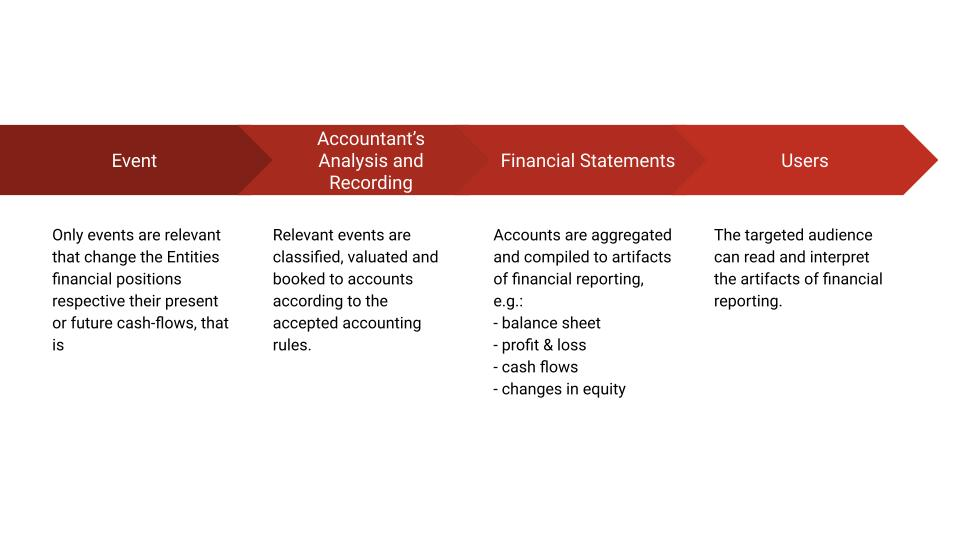
\includegraphics[width=0.7\textwidth]{../figures/Financial Accounting - fundamental relationships}
	\caption*{After \cite[p.3]{Horngren1984}: This figure indicates a process by setting general steps in an ordered relationship.} 
\end{figure}

The mentioned \enquote{accounting process} requires the identification of \enquote{transactions as they affect an organization}(\cite[p.13]{Horngren1984}).
Therefore \cite[p.13]{Horngren1984} introduces the entity as \enquote{specific area of accountability, a center of attention, a clear-cut boundary for reporting.}

The IASB Framework sets the entity as a reporting boundary:\cite[1.13]{IASBFramwork}

\blockquote{Information about the nature and amounts of a reporting entity’s economic resources and claims can help users to identify the reporting entity’s financial strengths and weaknesses. That information can help users to assess the reporting entity’s liquidity and solvency, its needs for additional financing and how successful it is likely to be in obtaining that financing. That information can also help users to assess management’s stewardship of the entity’s economic resources. Information about priorities and payment requirements of existing claims helps users to predict how future cash flows will be distributed among those with a claim against the reporting entity}

\cite{IASBFramwork} 

\blockcquote[3.4]{IASBFramwork}{Financial statements are prepared for a specified period of time (reporting period) and provide information about:
\begin{itemize}
	\item[] (a) assets and liabilities—including unrecognised assets and liabilities—
	and equity that existed at the end of the reporting period, or during
	the reporting period; and
	\item[] (b) income and expenses for the reporting period
\end{itemize}
}

\blockcquote[3.10]{IASBFramwork}{A reporting entity is an entity that is required, or chooses, to prepare financial statements. A reporting entity can be a single entity or a portion of an entity or can comprise more than one entity. A reporting entity is not necessarily a legal entity}

Imporatant is to distinguish between a company and its owner. In financial accounting, the company is the legal entity and therefore defines the point of view and the owner has rights on the companies assets.


% Usually a entity in this context is equivalent to a company.
Financial accounting always uses this boundary "what happens within my companies" but is never really reflecting other entities, besides 3rd parties in ageing lists.
Usually an entity represents a company and only this company.
Owners capital is reflected as equitiy and investments in other companies are usually subsumed as financial assets.
The entity acts therefore as point of view where only present and future financial transactions affecting the entity are in scope.
Both refer to the term \enquote{Entity} (also refer to as company, organization ) as subject, that sets the point of view and als the boundary for events relevant for Financial Accounting.
\todo{Insert Venn Diagram for Events: General Event, Business Event, Financial Event}

\subsection{Recognizable elements of financial statements}

\todo{Indicator for control over a resource: Present and future Cash flows as very important indicator }
Eingehen darauf, was wann erkannt wird: z.B. Fokus nicht nur auf Ereignisse das Unternehemn betreffend sondern ganz explizit mit direkten finanziellen Auswirkungen. (Einengen der Entity)
Weiter machen mit dem generellem Zeitpunkt des Erkennens

\todo{IASB 4.1 and 4.2 }

\todo{REcognition criteria IASB 5.6}

\todo{Horngren p. 13 - Transactions as exampel}


\begin{table}
	\caption{The elements of financial statements}\label{tab:elementsfinancialstatements}
	\begin{center}
% \begin{tabular}{|p{0.3\textwidth}|p{0.15\textwidth}|p{.5\textwidth}|}
	\begin{tabular}{|p{3,5cm}|p{2cm}|p{7,1cm}|}
	\hline
	Economic resource &
	  Asset &
	  A present economic resource controlled by the entity as a result of past events.
	  
	  An economic resource is a right that has the potential to produce economic benefits. \\ \hline
	Claim                                          & Liability & A present obligation of the entity to transfer an economic resource as a result of past events. \\ \cline{2-3} 
												   & Equity    & The residual interest in the assets of the entity after deducting all its liabilities           \\ \hline
	Changes in economic resources and claims, reflecting financial performance &
	  Income &
	  Increases in assets, or decreases in liabilities, that result in increases in equity, other than those relating to contributions from holders of equity claims. \\ \cline{2-3} 
	 &
	  Expense &
	  Decreases in asssets, or increases in liabilities, that result in decreases in equity, other than those relating to distributions to holders of equity claims. \\ \hline
	Ohter changes in economic resources and claims & -         & Contributions from holders of equity claims, and distributions to them.                         \\ \cline{2-3}
												   & -         & Exchanges of assets or liabilities that do not result in increases or decreases in equity.      \\ \hline
	\end{tabular}
	
\end{center}
	\caption*{This table from \cite[Section 4.2]{IASBFramwork} gives an overview of different elements that are recognized in financial statements.}
\end{table}








\section{Measurement and Valuation}


% \todo{IASB 5.4}


As mentioned in previous section \ref{sec:Finacc-Picture} accounting can be understood as "continuos, permanently changing picture" of an Entities resources.
To be able to "paint" this picture a process to 
Hier den Prozess skizzieren\dots




Financial accounting is often referred to as methodology to give an insight over the financial position of a company\dots
% \todo{Weiter ausarbeiten: Die Entity als Eventhorizont, Events als Auslöser von Veränderungen, Sichtweisen von Financial accounting (Moxter)}


In this chapter aspects of financial accounting most relevant for this thesis are introduced.
Most of interest are aspects that concern of a perspective of Accounting as a processing of events combined with the view from within a company as subject.
There are:k
\begin{itemize}
	\item Event recognition - are events relevant for entity.
	\item Event classification
	\item Event valuation
	\item 
\end{itemize}
\section{Profit \& Loss and the concept of accrual}
\section{Accounting Theories}

Although financial accounting and double entry accounting is known used since medieval formal standards barely existed until beginning of the 20th century.
Three different financial theories (dogmas) are summarized in \cite{moxter1984BilanzlehreI}, namely the 



Task: - find sufficient conecepts to map the REA data model to classical double entry book keeping.
-- use dynamische Bilanz for that purpose because:
-- Balance sheet entries are floating posts that are only temporary as soon as the business transaction is finished
-- Same IDEA for REA: A REA transaction is done, when all events for this transaction is done
-- At the end of the entity all floating items have to be resolved, if a company is shot down there never are unresolved items in a balance sheet. (and also not in the balance sheet at the start (except equity))


Moxter has three different Financial Accounting Theories

Moxter beschreibt in \cite{moxter1984BilanzlehreI} verschiedene Herangehensweisen.

Statische Bilanz => Ausgehend vom Vermögen
Dynamische Bilanz => Ausgehend von G\&
V (Siehe Beispiel einer kurzlebigen Unternehmung)



\section{Basic Picture of Accounting - Valuation \& Recognition Financial Accounting as process}





and introduces the concept of principals and surrogates to do a projection of real wordl predicates to a complete projection, that is all events that are relevant (for an entity) can be found in that view (in this case accounts).
Picture: Projection

Valuation by Rules Ijiri Page 94f.


The company in Financial Accounting is reflected as closed entity that has control over resources.
Measurment happens by events that change the control over resources.


While Financial Accounting is a stedy process of Recognition of 




\subsection{Three concepts}
Base for this projection is always the event horizon of an entity, I want to elaborate on three important concepts:

\subsection{Event horizon of the Entity}

\subsection{Resource and the axiom of control}

\subsection{Events that affect the resources under control}


\subsection{Process of Accounting}
Horngreen summarizes the process as follows, 

Measurement -> Brücke zu Ijiri

Classificational vs. Causal accounting


\section{Aspects of dynamic accounting in connection to REA}

Diese DA behandelt zwar "nur" die Buchhaltungstechnik, es scheint aber sinnvoll die Perspektive der dynamischen Bilanztheorie einzunehmen,
da "Ereignisse" in REA im weitesten Sinne eine Veränderung im Bestand verursachen und daran eine Analog gezogen werden kann.

%\item Dynamische Bilanz -> verschiedene Fälle







\section{The purpose of financial Accounting}
After Horngren, Accounting in general is the profession executed by Accountangs to \enquote{design their system after considering the types of information desired and other users}.\cite{Horngren1984}[p.3]
The desired informations are commonly used to answer questions after the perfomance of a \enquote{organization} in a given period and the (financial) standing in a certain moment in time.\cite{Horngren1984}[p.3]

\section{Artefacts in Financial Accounting}

\subsection{Debit and Credit}
=> Debit und Credit sind nur Begriffe 

Ijiry (as additional source) states that \enquote{Accounting is a system for communicating the economic events of an entity}. \cite{Ijiri1967}[p.3]
That is \enquote{The economic events of an entity must be represented by an organized set of symbols which are suitable for communication}. \cite{Ijiri1967}[p.3]

The most resulting artifacts of financial accounting activity are the income statement and the balance sheet.
\enquote{To obtain these statements}

\todo{Ijiri surrogates}




An event get's recognized, then it must be analyzed if it is relevant for financial position of the entity / if it changes the financial position of the entity.
Then Measurment, then classification

\section{Relevenace of Events }
An Event has to as to affect the financial position to be recognized in accounting 

For this to be true everey event has to analyzed for it's implicatoins

First it h of the entity
Secon it's classification 

realizatoin

Different types of events:
Business Event
Financial Event










\section{Causal accounting}

2021-09-12

This thesis considers two approaches to the basics of financial accounting.



+++++++

Excerpt: How can the consumption of services be modelled?

Intro: Horngren argues that every purchase of service as expense goes through balance sheet:
- Purchase on Assets for immediate consumption
- Consumption of service as expense
=> It is a kind of depreciation

In REA the first booking is easy:
Resource Money is exchanged against resource "Service".
But then this "Service" has to be consumed against what?

But: The benefit of "Service" stays inside the company, is it a kind of depreciation?
So this could be modeled as a pure financial event.

+++++++



The understaning of doing business and measuring the success has drastically changed over the past years.
Companies are required to deliver financial information at any time.
Thinking of Italian traders in the medieval age the motivation to account business transactions then today:
Back then it was usual to not have an annual closing, they rather calculated the success of a long lasting trade trips on a per trip base over years as Eugen Schmalenbach states:

\blockquote[\cite{schmalenbach1962}][]{Hier das Zitat!!!}

The trader did business on his own and a sum up was done after all related transactions where finished.
So there was no need to distungish between the owne and the company and also no need for accruals.

Schmalenbach starts with a hyphotetic business that lives only for a single purpose and is rolled up after this purpose is over.
The business gets credit from banks 
Within the lifetime of this company only incomes and expenses measured and at the end a single balance sheet is created:
All 
This balance sheetare aufgelöst after the purpose of this company i

Unterscheidung Aufwand und Ausgaben


Financial accounting took a long way from medeval ages where the economic success was calculated by economic long term project there was no difference between. Success was calculated after a cruise accross the ocean was finished on per project base, a yearly financial statement was unkown and not in focus.

Time after time and as money markets arised it was more and more important to give a complete view.


Following these requirements the P \& L oriented structured balance sheet 

A financial statement has to fullfill many requirments: It should give Investors an insight

Over time a company is considered as independent 










As kind of grounding of this thesis foundations of Accounting are investigated in this chapter.
The starting point is an overview over the process of accounting and fundamental terms of accounting, the main source for that part will be \cite{Horngren1984}.
Then fundamental connections between events, resources and following implications for measurment, classification and valuations are considered, this part will heavily rely on \cite{Ijiri1967}.
At last IFRS as concrete standard for measurement and classification is introspected as this will be the basis for mapping activities between the REA Data Model and financial accounting artefacts.
starting with the process of accounting, going further to typical artefactes and an analysis of mechanics in accounting.

The well known double entry accounting with it's first written introduction in \ldots by \ldots is widely anticiptated. % and worldwide used.
\enquote{Accounting is the major means of communicationg about the financial impact of an organzation's activities.}\cite[p.3]{Horngren1984}
It's
It's main artefacts are t-accounts, journals and as core the so called ALE Equation.

But what is behind the scenes?


To make rational choices, comprehensive information about a companies wealth to interested actors / audience is crucial.
Financial Accounting supports these decisions by delivering an overview over a companies assets and liabilities and Accrual Accounting extends this support by making the companies performance in a given period visible.

This chapter introduces fundamentals of Accounting and presents the audience and their benefits of the accrual accounting artefacts and relates fundamental concepts of accrual and further IFRS accounting to REA\textcopyright accounting.
% The outcome will be an answer, if the REA Accounting Model is feasable to 

Scope: Financial Accounting -> financial reporting: e.g. values of assets, cash, income-statement

Financial Reporting as statutary reporting

Historical: Accounts where closed when , there where 

We mean financial reporting as statutory reporting as it is needed to inform Owners, Creditors and tax authorities that has to be done at least once a year and structured as defined by laws or regularities

History of accounting\dots
Balance sheet was rather a Reume over projects (like sailings) rather than a regulary executed task.
Often a balance was taken when the main journal was full and a new book was startet.

Intention of balance sheet:
Overview over capital
Calculation of Earnings in a period
Schmalenbach calls this a dynamic balance, where in dopik the Profit \& Loss account is embeded between to balances.

Historicaly there was a lot of discussion about valuation of items, higher taxrates e.g. yield to a motiviation to minimize wealth and financial result to tax optimization.
The only intention of analysis financial accounting in this thesis is solely technical based.

There are different kind of events possible: once that are relevant for the business but not for finincial reporting, events that are relevant also for financial accounting and events that only exist to have propber visible accounting e.g. events that are deducting assets or to do the annual closing.



Start with cash -> then accrual


% \enumerate{}
Stake holders, why do we do accounting: Investors
Accounting terms: Entity, Transaction, Valuation, Measurement
Transaktion starts with events.
Events can be relevant for Business, or have a financial impact (beispiel ijiri manager)
Duration of events (ijiri?)

\section{The process of accounting}
Process of accounting: recognizing an event relevant for financial accounting, valuation

\begin{figure}
	\centering
	\caption{Process of Accounting}
	\label{fig:accounting-process}
	\includegraphics[width=0.7\linewidth]{"../figures/replace/CollaborativePerspective"}
	\caption*{Taken from \cite[p.3]{horngren2006introduction}. This figure }
\end{figure}


\section{Foundations of Accounting}
REA itself is an accounting model but let's recap what the most important
properties of accounting are. \todo{citation! to REA Paper}

These foundations of accounting provide the grounding for the following check of common properties and possibilities for wmapping.

\subsection{The Entity}
The entity represents the event horizon of an Financial Accounting System.
An Entity can be a company, a department or also a group of companies and an Financial Accounting system must be assigned to exactly one.
Everything that touches the financial positions of an corresponding (zugehörig) entity is recorded.
Everything else is ignored.\cite[p.15]{Horngren1984}

If an employee gets sick that possibly leads to damage (e.g. by delaying projects) to the entity but this event will not yet find it's way to a Financial Accounting System as he will be receiving is usual salaries.
For paid leaves there is a need to build a provision in case the employee leaves the entity and can not consume his quota.
So when he is going on holidays this will be reflected in Financial Accounting as the quota is reduced.

REA itself was also designed as entity centric accounting system but then extended to an \enquote{Open-edi Business Transaction Ontology (OeBTO)}\cite[Figure 2]{ISOIEC1594442015}\ref{fig:collaborative-perspective}.
Although the concepts of REA allow a wider view on Accounting systems in this thesis the \enquote{Trading Partner View} is used as there exists no collaborative spac in Financial Accounting Systems and to make the mapping between Financial Accounting and REA Accounting simpler and support better understanding.
As preview, it is preferable that events relevant for Financial Accounting are depicted either as \enquote{credit} or \enquote{debit} as shown in \cite{schwaiger2015aleandrea} and make sense only from the entity's point of view.

% \begin{figure}
% 	\centering
% 	\caption{REA Collaborative Perspective}
% 	\label{fig:collaborative-perspective}
% 	\includegraphics[width=0.7\linewidth]{"../figures/replace/CollaborativePerspective"}
% 	\caption*{Taken from \cite[Figure 2]{ISOIEC1594442015}. This figure demonstrates the two possible point of views that can be used. In this thesis the collaborative space is not relevant therefore the \enquote{Trading Partner View} is used.}
% \end{figure}

\subsection{Purpose of accounting}
Audiences
Scope of accounting: Support of Decisions, AUD IT GAAP => Tax
\subsection{Recognition of Events}

Accounting is generally speaking the process of recognizing relevant event, to analyse and store them and finally create financial statements that can be interpreted by interested audience.
What kind of events and when they are in scope of finance accounting is

Financial accounting stores only interpreted and aggregated data in monetary units whereas REA recognizes the events with all their attributes itself.
McCarthy calls this the \enquote{essence of events}\todo{citing}.
Figure \ref{fig:EventsTimeOfRecording} shows the process of accounting and compares the moment of recognition through in financial accounting and REA accounting in a timeline.
It must be considered, that not every
\begin{figure}
	\centering
	\caption{Time of recording in Accounting systems}
	\label{fig:EventsTimeOfRecording}
	\includegraphics[width=0.7\linewidth]{"../figures/EventsTimeOfRecording"}
	\caption*{This figure after \cite{Horngren1984} shows the different moments in time when recording happens. Traditional accounting first interprets the event and records the interpretation whereas REA stores all needed information of an event to interpret it afterwords.}
\end{figure}

\subsection{Management and Financial Accounting}
Purpose of accounting: Targeted Audience, difference between management and
financial accounting
\section{Concepts of Financial Accounting}
\subsection{The Statement of Financial positions}
The statement of financial positions is also called \enquote{balance sheet} as this equation has always to be true:
\[ Assets = Equities \]
The Assets consist of resources, that are under the equities control and the Equities can be further distinguished to:
\[ Equities = Liabilities + Shareholders equity\]


Different Types of Assets:

Tangible \& Intangible

Financial Assets

Direct tradable Assets acting as resources: Tangible \& intangible Assets,
Inventories, Cash

Discussion of Claims

Assets have nature of commitmens of other companies for future resource flow

Problem: Commitments can not be exchanged but this is possible with Assets that have only one borrower

\subsection{Liabilities}
Claim not feasable

Commitment

\subsection{The income statement}
Accrual accounting here\ldots

Development of equation

Debit / Credit

Changes in Equity\ldots

Different Types of bookings:
Even Services are in fact

=> Events that have effect to income statement and events that have not.

Accrual Accounting: Revenue and Expense are connected

2 Beispiele: Kauf von Verbrauchsmaterial => 1) Sofortige Abschreibung 2) Kauf auf Lager, dann Verkauf => Muss bei Mapping von Events berücksichtigt werden / Oder hängt es an der Resource? Lagerresource vs. Verbrauchsresource Inventoryresource vs. consumables

\section{Accrual Accounting}
Special ledgers: Creditors, Debitors, Ageing




\section{IFRS Accrual Accounting}
Usual artefacts out of IFRS Accounting: Balance Sheet, Income Statement, Changes in Equity, Cash Flow
Other usefull artefacts: Ageing list by business partner,


More or less interresting for valuation and recognition, not technical
modelling.

Will be used for Case study\ldots




\begin{table}
	\caption{}\label{tab:Elementary concepts}\caption*{}
	\begin{tabular}{|p{0.15\linewidth}|p{0.15\linewidth}|p{0.15\linewidth}|p{0.55\linewidth}|}
		\hline
		Categorie & Accrual Accounting & REA\textcopyright{} Accounting & Analysis result
		\\
		\hline
		Scope     & Entity             & REA Internal View              & REA itself can be used from an outside or
		inside entities viewpoint. In this thesis the internal viewpoint is
		choosen
		\\
	\end{tabular}
\end{table}

\section{Summary}
In this chapter the foundations of Financial Accounting and the resulting ALE Datamodel where presented.
The Event based character of Financial Accounting was studied and the process behind that leads to this Datamodel was analyzed.

It was pointed out, that conceptualy double entry accounting is a surrogate for real events, so every booking represents an event identified as relevant to an entities financial positions.

The \enquote{Double Entry Accounting} is a common notation for an \enquote{ALE Date Model} that technicaly stores these analyzed events on the \enquote{debit} or \enquote{credit} side of an Account so that the \enquote{ALE Equation} holds.
Nevertheless especially \enquote{debit} and \enquote{credit} don't hold any semantic meaning and are merely technical terms to acomplish this restriction and their interpretation depends on the class of the booked Account.

The dynamic nature of \enquote{Accrual Accounting} was explored and also the impact of past, present and future events.
Different Accounting Theories and their different views on Financial Accounting where outlined.

Also the difference between classificational and causal accounting was discussed, whereas in causal accounting every change in financial positions is connected to an event that causes that change.

With this knowledge about the mechanics behind Financial Accounting a mapping will be done in Chapter 3 \todo{Insert reference}.